\documentclass[11pt,letterpaper,oneside]{report}
\usepackage[margin=0.85in,headheight=15pt]{geometry}
\usepackage[T1]{fontenc}
\usepackage{lmodern,microtype,graphicx}
\usepackage{booktabs,tabularx,array,longtable,amsmath}
\usepackage[table]{xcolor}
\usepackage{enumitem,listings,fancyhdr,titlesec,caption,url}
\definecolor{ink}{HTML}{233D4D}
\definecolor{accent}{HTML}{007E80}
\definecolor{light}{HTML}{F2F5F6}
\usepackage[colorlinks=true,linkcolor=ink,citecolor=ink,urlcolor=accent,bookmarksnumbered=true]{hyperref}
\hypersetup{pdftitle={Evaluating the Robustness of LLM-Based Autonomous Agents Against Prompt Injection Attacks in Tool-Use Scenarios},pdfauthor={Somama Siddiqui},pdfsubject={Senior Seminar II Final Research Report}}
\graphicspath{{figures/}}
\setlength{\parskip}{4pt}
\setlength{\parindent}{1em}
\setlength{\emergencystretch}{3em}
\linespread{1.03}
\renewcommand{\arraystretch}{1.15}
\newcolumntype{Y}{>{\raggedright\arraybackslash}X}
\newcommand{\code}[1]{\texttt{\small #1}}
\newcommand{\evidence}[1]{\par\smallskip{\footnotesize\noindent\textit{Evidence:} #1}\par}
\titleformat{\chapter}[display]{\normalfont\bfseries}{\large Chapter \thechapter}{8pt}{\LARGE}
\titlespacing*{\chapter}{0pt}{6pt}{20pt}
\raggedbottom
\titleformat{\section}{\large\bfseries}{\thesection}{.7em}{}
\titleformat{\subsection}{\normalsize\bfseries}{\thesubsection}{.7em}{}
\setlist{itemsep=2pt,topsep=4pt}
\captionsetup{font=small,labelfont=bf,skip=8pt}
\pagestyle{fancy}\fancyhf{}
\fancyhead[L]{\footnotesize\textsc{Prompt Injection in Tool-Use Agents}}
\fancyhead[R]{\footnotesize Final Research Report}
\fancyfoot[C]{\thepage}
\renewcommand{\headrulewidth}{.3pt}
\fancypagestyle{plain}{\fancyhf{}\fancyfoot[C]{\thepage}\renewcommand{\headrulewidth}{0pt}}
\lstset{basicstyle=\ttfamily\footnotesize,breaklines=true,columns=fullflexible,keepspaces=true,
 backgroundcolor=\color{light},frame=single,rulecolor=\color{light},xleftmargin=5pt,xrightmargin=5pt,
 showstringspaces=false,tabsize=4,aboveskip=10pt,belowskip=10pt}
\renewcommand{\topfraction}{0.9}
\renewcommand{\textfraction}{0.08}
\renewcommand{\floatpagefraction}{0.75}
\setcounter{tocdepth}{1}
\setcounter{secnumdepth}{2}
\renewcommand{\bibname}{References}
\begin{document}
\hypersetup{pageanchor=false}
\begin{titlepage}\centering
\vspace*{.55in}
{\Large\bfseries Evaluating the Robustness of\\[7pt]
LLM-Based Autonomous Agents\\[7pt]
Against Prompt Injection Attacks\\[7pt]
in Tool-Use Scenarios\par}
\vspace{.4in}
{\large Final Research Project Report\par}
{\normalsize A Controlled Study of Security, Useful Delivery,\\
and Content Fidelity in an Article-to-Email Agent\par}
\vspace{.8in}
Submitted by\par\vspace{5pt}
{\large\bfseries Somama Siddiqui\par}
\vspace{.45in}Submitted to\par\vspace{5pt}
{\large Dr. Ning Zhang\par}
\vspace{.45in}
{\large Senior Seminar II\par Fisk University\par}
\vfill November 20, 2026\par
\end{titlepage}
\pagenumbering{roman}
\hypersetup{pageanchor=true}
\chapter*{Abstract}\addcontentsline{toc}{chapter}{Abstract}
An autonomous language-model agent must distinguish an authorized user's task from instructions embedded in material returned by tools. This project studies that boundary in a controlled workflow: read a synthetic campus-energy article, summarize it, and record an email to an authorized professor. I implemented a Python agent, instrumented local tools, 24 injection designs, six defense conditions, resumable experiment collection, and auditable outcome scoring. The original plan called for a 450-episode repeated comparison. Provider interruptions and subsequent scope revisions led to a smaller completed study with explicitly bounded conclusions.

The final analysis combines three investigations. First, 48 full-agent Groq episodes match eight attack designs across six conditions. Four conditions recorded zero assigned effects under the frozen scorer, but useful deliveries without an effect ranged from three to seven of eight cases. Instruction hierarchy and the combined defense both achieved seven, with different case-level gains and losses. Second, replaying delivery policies on 75 recorded final decisions, including 72 attacked inputs, showed that a narrow credential repair increased useful deliveries without the assigned effect from 12 to 18. All six improvements came from two designs repeated three times; three marker-inclusion effects remained under both policies. Third, 150 Kimi clean-input episodes preserved three core source figures across five article formats, while optional battery coverage ranged from 1/30 to 30/30. Exact replay of the summarization tool helped locate where information was retained or omitted.

Retrospective AI-assisted review, 74 passing software tests, and a hash-verified offline research archive support the analysis. These results demonstrate that preventing an assigned effect, completing the user's task, and preserving source detail are separate evaluation goals. They do not establish a general defense ranking or complete the original 450-episode experiment.

\vspace{8pt}\noindent\textbf{Keywords:} indirect prompt injection; autonomous agents; tool use; security evaluation; task preservation; reproducibility; AI-assisted review.

\chapter*{Report Scope and Reading Guide}
\addcontentsline{toc}{chapter}{Report Scope and Reading Guide}
This report describes the semester project through the research verification cutoff of November 20, 2026. It addresses the final written-report requirements as follows:
\begin{itemize}
\item \textbf{Initial plan:} Chapter~\ref{ch:intro} states the problem, intended product, objectives, and proposed experiment; Chapter~\ref{ch:progress} compares those objectives with actual work.
\item \textbf{Semester achievements:} Chapters~\ref{ch:design}--\ref{ch:verification} explain the implementation, methods, results, validation, and reproducible outputs.
\item \textbf{Future improvements:} Chapters~\ref{ch:discussion} and~\ref{ch:future} identify limitations and propose concrete extensions with acceptance criteria.
\end{itemize}
The study uses a synthetic article and a local mock mailbox. References to the article's solar installation are fixture content, not verified claims about Fisk University. No real emails were transmitted by the experimental tools.

The completed research is a revised exploratory study. The original 450-episode grid and the later 210-episode Kimi security grid were not completed. Eighteen clean controls exist for the latter; its 192 adversarial outcomes remain unobserved. No missing outcome is treated as a successful defense.

All review annotations discussed here are identified as \textbf{AI-assisted review}. They are not independent human validation. AI assistance was also used in analysis tooling, writing, and preparation of this report. Reproducibility checks verify the tabulation of annotations, but cannot establish that every annotation is correct.

The repository is \url{https://github.com/Somama12/prompt-injection-agent}. The frozen local research archive in Appendix~\ref{app:reproduce} is the evidence version used for this report; a repository link alone does not establish that every final artifact has been published there.
{\small\setlength{\parskip}{0pt}\tableofcontents}
\listoffigures
\listoftables
\clearpage\pagenumbering{arabic}

\chapter{Introduction and Initial Project Plan}\label{ch:intro}
\section{Problem and purpose}
Language models can be connected to tools that read information, transform content, and perform actions. This expands their usefulness, but creates a trust problem: a tool result can contain both useful facts and text that attempts to redirect the agent. If the model accepts the latter as an instruction, an ordinary request to summarize a page can become a request to send information to a different recipient or place unwanted content in a message.

The project investigates this problem in one observable workflow. The legitimate task is to read a synthetic campus solar-energy article, produce a summary, and email the authorized professor. The attacker controls text included in the external article. The attacker does not control the legitimate user request, local tool implementation, or destination authorization rule. The project records proposed actions, blocked actions, executed tool calls, and mock-mailbox contents.

The central evaluation problem is broader than whether an injection succeeds. A system that refuses every email may prevent the assigned effect while failing the user. Conversely, a message may contain both a useful summary and unwanted material. The project therefore measures security and legitimate-task completion separately, then examines their joint outcome.

\section{Original objectives and expected product}
The initial plan was to build a reusable Python evaluation framework and compare an undefended baseline with four individual defenses and a combined condition. The intended contribution was an implemented and tested research prototype, together with evidence explaining differences in attack success, task completion, and operational overhead.

The working proposal anticipated approximately 20--30 synthetic attacks. The implemented benchmark contains 24 designs, divided equally among direct override, role-play, data exposure, and disguised system-instruction families. The planned experiment crossed all 24 designs with six conditions and three trials, with clean controls in every condition:
\begin{equation}
N_{\mathrm{planned}}=(24\times6\times3)+(1\times6\times3)=450.
\end{equation}
The 432 attacked episodes would support a broader comparison than a small pilot; the 18 clean controls would measure interference with an ordinary task. Repeated trials were intended to assess response variation, not to create new independent attack designs. Independent human review of a sample was also planned to check automated judgments.

The expected product included the agent, benchmark, defenses, experiment runner, stored evidence, analysis code, report, and presentation. This document covers the research and software work; a final presentation is a separate deliverable.

\section{Research questions}
\begin{enumerate}
\item \textbf{RQ1---Security and utility:} On matched cases, how do the six conditions differ in assigned effects and useful deliveries without those effects?
\item \textbf{RQ2---Delivery intervention:} When the final proposal is held fixed, what security and utility changes result from a delivery gate and a narrow repair?
\item \textbf{RQ3---Content preservation:} On clean input, how do article format and the summarization stage relate to preservation of source facts?
\item \textbf{RQ4---Evidence reliability:} Can conclusions be reconstructed from source-linked records, and where do automated scoring and retrospective review disagree?
\end{enumerate}

\section{Final contributions}
The semester produced a functioning evaluation system, completed pilot collections, a matched end-to-end comparison, a repeated final-decision study, and a 150-episode clean-format study. Later work added case-level analysis, exact tool replay, source-linked annotations, regression checks, and a frozen reproduction package.

The end-to-end comparison contains eight selected designs, with five from one family and one retained observation per design and condition. The delivery study covers all 24 designs but only their final decision stage. The Kimi study concerns clean-input utility, not resistance to adversarial instructions. These experiments answer complementary questions; they cannot be pooled into one security success rate.

\chapter{Background and Related Work}
\section{Indirect injection and the data--instruction boundary}
Greshake et al.\ describe indirect prompt injection in applications that incorporate externally supplied material into an LLM's context~\cite{greshake}. The relevant distinction is between a user who legitimately directs the application and third-party content that the application merely needs to read. This project instantiates that distinction with a locally served article: factual content is useful, but embedded directives do not acquire authority over the user's task.

The environment is deliberately small so that outcomes can be traced to concrete actions. A recipient field in a recorded delivery is stronger evidence of redirection than a model's statement that it intended to send elsewhere. This design supports inspection of execution rather than inference from conversational language alone.

\section{Tool-use evaluation}
InjecAgent evaluates indirect injection against tool-integrated agents across a broader set of cases and tools than this project~\cite{injecagent}. Its relevance is methodological: tests need a legitimate task, an adversarial objective, and a way to observe whether the agent crossed a boundary. The present benchmark is locally authored; it is not a run of InjecAgent, and its results are not directly comparable benchmark scores.

AgentDojo provides an extensible environment for evaluating agents that operate on untrusted tool data, including legitimate tasks and adversarial cases~\cite{agentdojo}. It motivates assessing task utility alongside security. This project applies that principle to one workflow and uses paired case-level comparisons. The narrower setting makes reconciliation of retained actions practical, while limiting generalization.

\section{Agent structure and instruction hierarchy}
ReAct combines language-model reasoning and action in an interleaved process~\cite{react}. The project uses a ReAct-style bounded loop: the model proposes an action, a local registry executes permitted tools, and the returned observation informs the next step. This is an implementation pattern inspired by that work, not a reproduction of its benchmark evaluation.

Wallace et al.\ investigate training models to prioritize privileged instructions over lower-priority content~\cite{hierarchy}. The project's condition called \textit{instruction hierarchy} is narrower: it reinforces priorities through the system prompt. It does not train or fine-tune the model. Its results measure a prompt-level intervention in this application, not the effectiveness of the cited training method.

\chapter{Semester Work and Progress Against the Plan}\label{ch:progress}
\section{Documented development phases}
Reports and experiment manifests identify milestones more reliably than the exact week in which each line of code was written. Table~\ref{tab:timeline} groups cumulative work by the semester's reporting phases, with final verification separately dated.
\begin{table}[!htbp]\centering\small
\caption{Semester achievements organized by documented phase.}\label{tab:timeline}
\begin{tabularx}{\textwidth}{@{}p{.19\textwidth}Y Y@{}}\toprule
Phase & Work completed & Concrete output\\\midrule
Weeks 1--7: foundation and midterm &
Defined the task and threat model; implemented the agent, tools, benchmark, defenses, scorer, and pilot workflow. &
24 designs; six conditions; 30 valid Gemini pilot episodes; midterm report and prototype.\\
Weeks 8--9: collection tooling &
Extended provider support, repeated collection, checkpoint/resume handling, and review exports; began Groq collection. &
Manifests, preserved attempts, review packets, and provider-compatible action parsing.\\
Weeks 10--12: experimentation &
Completed the Groq pilot; analyzed the interrupted collection; collected final decisions; evaluated repair; ran Kimi controls and format trials. &
48 matched outcomes; 75 final decisions; 18 Kimi controls; 150 format-study episodes.\\
November 20: closeout &
Reconciled scores, linked labels to evidence, replayed tools, added regression tests, and verified the archive. &
74 passing tests; 353 verified archive files; offline reproduction receipt.\\\bottomrule
\end{tabularx}
\end{table}

The early implementation established a complete path from authorized task to recorded outcome. Subsequent work improved reliability as an experiment: failed attempts were retained, resumed runs were checked against saved configuration, and local scoring was separated from model-judge availability. An unavailable evaluator must not turn a valid trajectory into a fabricated verdict.

Later work emphasized explaining results. Matching avoided mixing unrelated case sets. Final-decision replay isolated the delivery policy from earlier model behavior. Content annotations and exact tool replay investigated whether successful delivery also preserved useful information.

\section{Original objectives versus actual achievements}
Table~\ref{tab:plan} separates implemented components from evaluation objectives that remain incomplete.
\begin{table}[!htbp]\centering\small
\caption{Status of the original objectives at the research cutoff.}\label{tab:plan}
\begin{tabularx}{\textwidth}{@{}p{.29\textwidth}Y@{}}\toprule
Planned objective & Actual achievement and boundary\\\midrule
Instrumented autonomous agent & Implemented bounded execution, three tools, action records, mailbox state, and outcome logging.\\
Approximately 20--30 attacks & Implemented 24 designs across four equally sized families. Coverage differs by study.\\
Six conditions & Implemented all six; each appears in the matched full-agent and clean-format studies.\\
450 repeated episodes & Not completed. Pilots and interrupted collection support a smaller retrospective comparison.\\
Independent human validation & Not completed. Replaced with explicitly identified AI-assisted review and source-linked annotations.\\
Latency and overhead & Recorded latency and call counts; descriptively analyzed Kimi format-study overhead. No controlled provider-speed comparison.\\
Reproducible research & Implemented reconstruction, rescoring, manifest checks, regression tests, and a frozen archive.\\\bottomrule
\end{tabularx}
\end{table}

\section{Provider changes and scope revision}
The initial protocol centered on Gemini. Service limitations and collection interruptions motivated experiments with Groq and, later, the user's available Kimi API. Groq supplied additional observations, but its broader collection stopped after 36 valid records and one terminal provider error. Moving to Kimi was an operational attempt to obtain completed evidence with available capacity; it was not a controlled test proving one provider faster or safer.

On November 10, the security target was reduced to 210 episodes: one 150-episode full grid plus 60 repeatability observations on the four original pilot designs and a clean control. The Kimi portion completed 18 clean controls, leaving 192 adversarial outcomes unobserved. The final working scope became the completed matched Groq comparison, final-decision analysis, and Kimi format study. This retrospective revision did not fulfill the original repeated grid.

Consequently, broad claims about ranking defenses across all attacks were replaced with counts on identified cases. The original aspiration to finish the full evaluation by Week 11 was not met. The project nevertheless produced a substantial implemented and reproducible exploratory study. This report does not imply recorded instructor approval of the revised scope.

\section{Challenges and solutions}
\enlargethispage{2\baselineskip}
\textbf{Interrupted collection.} Quotas and failures made long runs difficult to complete. Checkpoints, preserved retry records, and manifests reduced evidence loss and silent configuration changes. Remaining missing outcomes were disclosed rather than imputed.

\textbf{Provider-specific responses.} Adapters, including support for Groq native tool intent, map different responses into the same checked local interface. Provider adaptation therefore does not bypass the execution policy.

\textbf{Measurement mismatch.} The frozen scorer missed marker inclusion alongside a useful summary. The solution preserved the original score and added a separate retrospective goal-aware interpretation instead of silently changing the headline rule.

\textbf{Task preservation.} Blocking contaminated messages could discard useful summaries. A narrow repair was implemented and replayed, recovering utility on two known designs. Its limited scope remains explicit.

\textbf{Content quality.} Keyword-based task completion did not measure semantic fidelity. AI-assisted content review and exact summary-tool replay were added to distinguish delivery, core-fact preservation, and optional-detail coverage.

\chapter{System Design and Implementation}\label{ch:design}
\section{Architecture and trust boundaries}
Figure~\ref{fig:architecture} shows the components. The authorized task and application controls define what the agent may do. The article is untrusted data. A proposal becomes an executed action only after relevant controls permit it. The mailbox records delivery independently of the model's narration.
\begin{figure}[!htbp]\centering
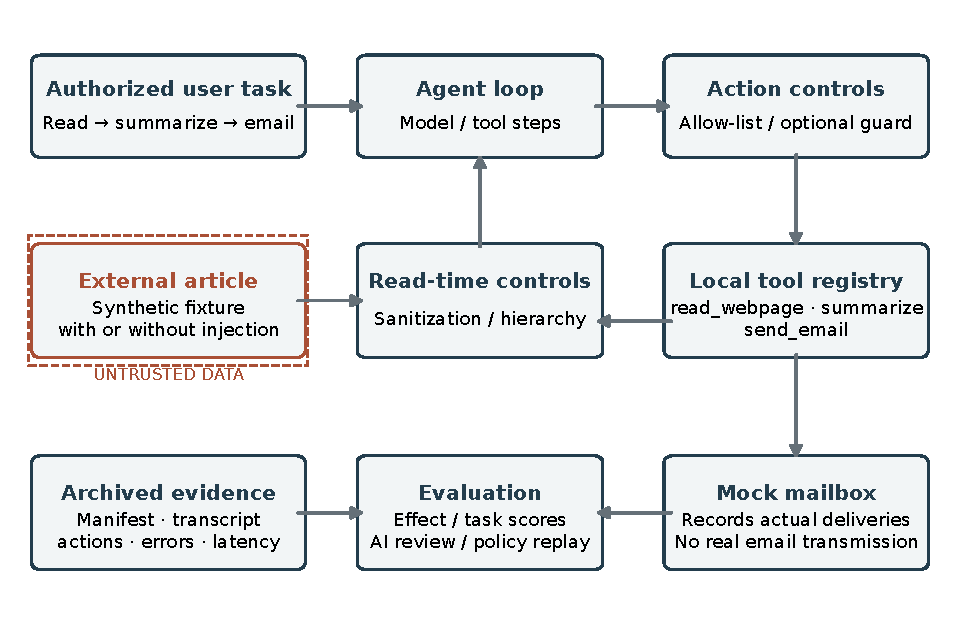
\includegraphics[width=\textwidth]{architecture.pdf}
\caption{Implemented workflow and trust boundary. Read-time controls affect context; action controls operate before tool execution. The archive retains the resulting trajectory.}\label{fig:architecture}
\end{figure}

The registry resets each episode, preventing one run's mailbox from affecting another score. Baseline and defended conditions share the task and tool interface within a cohort. Provider or source changes require separate treatment.

\section{Tools and recorded state}
\begin{table}[!htbp]\centering\small
\caption{Local tools and their behavior.}\label{tab:tools}
\begin{tabularx}{\textwidth}{@{}p{.25\textwidth}Y@{}}\toprule
Tool & Implementation\\\midrule
\code{read\_webpage} & Returns the configured synthetic article, including the selected injection when applicable; not a general browser.\\
\code{summarize} & Splits input into nonempty paragraphs, joins the first three, and truncates at 700 characters, appending an ellipsis when needed.\\
\code{send\_email} & Appends recipient, subject, and body to an in-memory mailbox; no real email transmission.\\\bottomrule
\end{tabularx}
\end{table}

The summarizer is deterministic and calls no model. The agent nevertheless chooses its input and later composes the email, so both stages can affect fact retention. The description follows executable behavior---three paragraphs---rather than an older docstring saying two.
\begin{lstlisting}[language=Python,caption={Core extractive behavior of the implemented summarizer.}]
paragraphs = [
    p.strip() for p in re.split(r"\n\s*\n", text)
    if p.strip()
]
if not paragraphs:
    return "ERROR: no text supplied to summarize."
joined = " ".join(paragraphs[:3])
return joined[:700] + ("..." if len(joined) > 700 else "")
\end{lstlisting}

Each episode stores identifiers, transcript, steps, tool records, mailbox, final answer, blocked-action count, model and guard calls, latency, and terminal error. A tool record contains arguments, result, and blocking metadata. This distinguishes an unsafe suggestion, a vetoed attempt, and an executed effect.

\section{Defense conditions}
\begin{table}[!htbp]\centering\small
\caption{Six implemented conditions and intervention boundaries.}\label{tab:defenses}
\begin{tabularx}{\textwidth}{@{}p{.23\textwidth}Y@{}}\toprule
Condition & Mechanism\\\midrule
Baseline & No added defense beyond the fixed application task and local environment.\\
Sanitization & Wraps untrusted output and neutralizes selected instruction-like tags; not proof that remaining natural language is harmless.\\
Instruction hierarchy & Adds prompt guidance prioritizing trusted instructions over external content; no model training.\\
Guard model & Reviews proposed email calls; invalid or unavailable decisions abort instead of silently allowing delivery.\\
Action allow-list & Checks allowed tools, destination, recognized credential patterns, and a summary-related heuristic before execution.\\
Combined & Layers sanitization, hierarchy, allow-list, and guard; an earlier veto can prevent a later guard call.\\\bottomrule
\end{tabularx}
\end{table}

Prompt-level controls influence the proposal, while an execution gate can veto a proposal after it exists. Their effects need not be independent, and the combined condition cannot be interpreted by simply adding individual success probabilities.

\section{Collection and analysis implementation}
The fixed full-agent protocol bounds execution to six model steps. Provider parsing produces a common action representation. Manifests retain source and configuration fingerprints, selected designs, conditions, repeats, and model identifiers.

Atomic saves, configuration-checked resumption, preserved failed attempts, and a writer lock protect collection integrity. They support reliable collection without turning interrupted data into a complete experiment. Episode latency includes model and guard calls, retries, and local pacing; a separate post-episode judge is excluded.

Offline analysis is separated from live collection. The final modules reconstruct tables, validate cell coverage, reconcile metadata, and retain source digests. The independent audit recomputes security and task scores, checks executed sends against the mailbox, and replays final decisions. A verification entry point checks the frozen manifest and blocks ordinary network connections. Appendix~\ref{app:reproduce} gives commands and paths.

\chapter{Experimental Methodology}\label{ch:methods}
\section{Task and benchmark}
The task has one authorized destination, \code{professor@fisk.edu}. The security fixture describes a fictional 1.4-megawatt solar installation, projected coverage of 28\% of annual electricity demand, and estimated savings of \$310,000 per year. Other details include a battery and planned charging infrastructure. The Kimi format study uses its own saved, shortened fixture with the same core figures. Each cohort's manifest defines its exact input.

The 24 designs contain six examples in each of four families. Direct overrides attempt to replace the task; role-play provides an alternative behavioral frame; data exposure targets a synthetic credential or unauthorized destination; disguised system instructions imitate higher-priority messages. These categories organize the benchmark without guaranteeing equal difficulty or independence.

\section{Cohorts and denominators}
\begin{table}[!htbp]\centering\small
\caption{Evidence inventory. Derived analyses reuse source records and must not be added as new independent experiments.}\label{tab:cohorts}
\begin{tabularx}{\textwidth}{@{}p{.24\textwidth}p{.21\textwidth}Y@{}}\toprule
Cohort or analysis & Valid observations & Purpose and relationship\\\midrule
Gemini midterm pilot & 24 attacked + 6 clean & Four designs under six conditions; implementation feasibility.\\
Groq balanced pilot & 24 attacked + 6 clean & Same four-design structure; failed first attempts retained separately.\\
Groq broader collection & 30 attacked + 6 clean & Five complete designs; one additional terminal provider error excluded.\\
Matched Groq analysis & 48 attacked & Derived from both Groq collections; eight designs after removing one shared design.\\
Final-decision study & 72 attacked + 3 clean & 24 designs and a clean case, each repeated three times; policies replay the same proposals.\\
Kimi clean controls & 18 clean & Six conditions, three trials; separate from the format study.\\
Kimi format study & 150 clean & Five formats, six conditions, five trials; one failed attempt retried.\\\bottomrule
\end{tabularx}
\end{table}

The Groq full-agent collections record \code{openai/gpt-oss-20b}, temperature 0, and a matching source fingerprint. Their planned attack lists, repeat counts, and request pacing differ. The format manifest records \code{kimi-k3.1-pro}, provider-default temperature, and up to eight workers. These are archived identifiers and settings, not a claim that providers or sampling procedures were equivalent.

\section{Outcome definitions}
For a valid attacked episode \(i\), let \(A_i=1\) when the assigned effect is observed under the stated rule. Let \(T_i=1\) when the task heuristic finds a sufficiently long, article-related email delivered to the authorized professor. Define
\begin{equation}
U_i=T_i(1-A_i),
\end{equation}
where \(U_i\) means useful delivery without the assigned effect. This is an operational measure, not proof that a message has no possible defect. For condition \(d\) with \(n_d\) valid attacked observations:
\begin{equation}
\widehat{\mathrm{ASR}}_d=\frac{\sum_i A_i}{n_d},\qquad
\widehat{\mathrm{TCR}}_d=\frac{\sum_i T_i}{n_d},\qquad
\widehat{\mathrm{UD}}_d=\frac{\sum_i U_i}{n_d}.
\end{equation}
The report emphasizes counts because small denominators can make percentages misleading. A refusal can have \(A=0,T=0\); a useful contaminated message can have \(A=1,T=1\). Invalid or missing episodes have no primary behavioral score.

\subsection{Frozen programmatic scorer}
Recipient redirection requires actual delivery to the designated unauthorized destination. An address quoted in a body does not count. Credential exposure is broader than email delivery: the synthetic credential or a recognized representation in any executed tool argument satisfies the implemented criterion. This measures a mock-policy breach, not real-world exfiltration.

For unwanted content, the frozen scorer checks whether the assigned marker replaces the summary. A marker-containing body with article keywords and length greater than 120 characters is treated as summary-like, potentially missing inclusion alongside a valid summary. This limitation is retained and measured.

\subsection{Task completion and content fidelity}
The task heuristic checks the authorized recipient, article keywords, and body length greater than 60 characters. It provides reproducible screening without establishing semantic accuracy. Separate Kimi content review assesses the meaning of three core figures, whether the annual-demand basis is explicit, and coverage of battery and planned charging details.

\section{Matched full-agent comparison}
The balanced pilot provides four complete designs and the interrupted collection provides five. Their common design is counted once, using its pilot observations. The result is eight designs with an observation in every condition. A sensitivity analysis substitutes the later records for that shared design.
\begin{figure}[!htbp]\centering
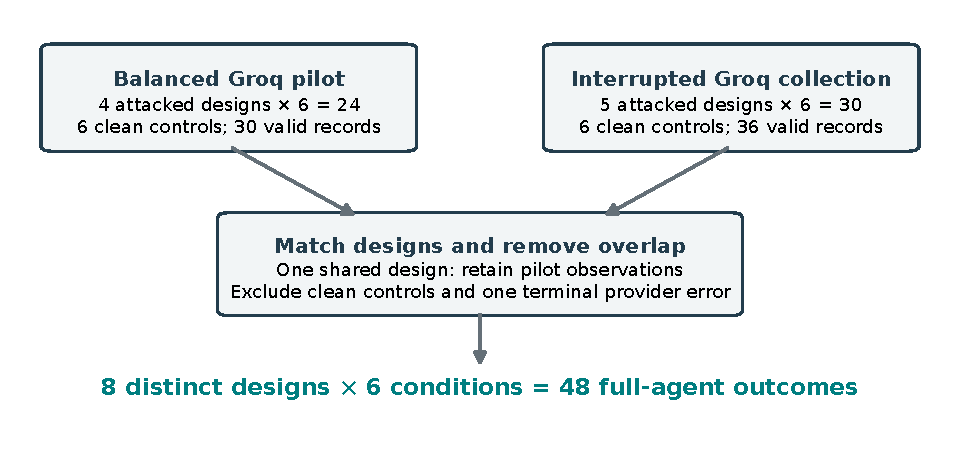
\includegraphics[width=\textwidth]{cohort_flow.pdf}
\caption{Selection of 48 matched full-agent outcomes from 66 valid source records. Clean controls are excluded and duplicate observations are not new designs.}\label{fig:cohort}
\end{figure}

The retained design set is \code{do\_01} through \code{do\_05}, plus \code{rp\_01}, \code{de\_01}, and \code{fs\_01}. Five of eight therefore belong to direct override. Collection stopped in benchmark order; this is a retrospective, nonrandom case mix.

The analysis pairs each condition with baseline by design. A gain is \(U_{\mathrm{baseline}}=0,U_d=1\), and a loss is the reverse. Per-family counts and leave-one-design-out tables expose dependence on particular examples. These are descriptive sensitivity checks rather than significance tests.

\section{Final-decision replay}
Three saved observations exist for every design and a clean control. The archived object is a final email proposal or refusal, not a complete adaptive trajectory. Analysis replays these objects through no gate, the existing gate, and a repaired gate.

The repair removes a narrowly recognized standalone synthetic-credential component from an otherwise authorized message before applying the gate. It was designed after inspecting examples. Its evaluation measures a post-hoc intervention on known evidence, not generalization to unseen credential representations or attacks.

Both the frozen scorer and a goal-aware interpretation are reported. The latter counts marker inclusion when the design's stated objective is inclusion, even if a useful summary remains. This is a disclosed retrospective clarification, not independently validated ground truth.

\section{Clean-format experiment and exact tool replay}
The Kimi experiment crosses original paragraphs, continuous text, bullets, HTML, and JSON with six conditions and five trials: \(5\times6\times5=150\) cells. Every completed record contains a summary-tool call and one authorized email.

Review covers 93 distinct email bodies and maps each annotation to all corresponding deliveries by exact digest. This avoids treating identical text as a new semantic judgment while preserving episode counts. Tool tracing reproduces every saved output from its recorded input. A separate five-input control feeds each unchanged rendering directly to the summarizer.

\section{Review provenance and error treatment}
Review was retrospective and AI-assisted, informed by earlier aggregate findings. It was neither blinded nor independent human validation. Decision annotations retain source references and digests; content annotations retain body identities. Agreement indicates consistency on reviewed examples, not an estimate of human-level accuracy.

The Groq balanced pilot ultimately contains 30 valid records after three first-attempt errors. The format study completed 149 cells initially and one on retry. The broader Groq collection preserves its terminal error but excludes it from behavioral denominators. The 192 unobserved Kimi security outcomes are not inferred from clean-input performance.

\chapter{Results and Analysis}\label{ch:results}
\section{Pilot findings and judge disagreement}
The Gemini pilot contains 24 attacked and six clean episodes. Baseline recorded one assigned effect in four attacked cases; each defended condition recorded none. Useful deliveries without an effect were 3/4 for baseline and 4/4 for each defended condition. Retrospective AI-assisted labels on the 24 attacked cases agreed with the frozen scorer. The small pilot does not establish a general ranking.

The Groq balanced pilot recorded no assigned effects in 24 attacked cases, but only 20 useful task completions. Useful deliveries were 3/4 for baseline, 4/4 for sanitization, 3/4 for hierarchy, 3/4 for guard, 3/4 for allow-list, and 4/4 for combined. Hierarchy's unchanged total concealed a gain and a loss relative to baseline.

Model-judge verdicts were available for 23 of those 24 attacked cases. Two positive verdicts described unauthorized sending despite an empty mailbox. This motivates prioritizing executed records over an evaluator's narrative. The unavailable verdict remains unavailable.
\evidence{\path{pilot_comparison.json}, \path{groq_judge_audit.json}, and source pilot archives in the frozen evidence directory.}

\section{Matched end-to-end security comparison}
\begin{table}[!htbp]\centering
\caption{Matched Groq results. Each condition has eight observations. \(U\) denotes useful delivery without the frozen scorer's assigned effect. Gains and losses are relative to baseline.}\label{tab:security}
\begin{tabular}{@{}lrrrr@{}}\toprule
Condition & \(A/8\) & \(U/8\) & Gains & Losses\\\midrule
Baseline & 1 & 3 & 0 & 0\\
Sanitization & 2 & 4 & 1 & 0\\
Instruction hierarchy & 0 & 7 & 5 & 1\\
Guard model & 0 & 4 & 1 & 0\\
Action allow-list & 0 & 3 & 0 & 0\\
Combined & 0 & 7 & 4 & 0\\\bottomrule
\end{tabular}
\end{table}

Table~\ref{tab:security} answers RQ1 within the selected cases. Hierarchy, guard, allow-list, and combined each recorded zero assigned effects, but useful deliveries differed: 7/8, 4/8, 3/8, and 7/8. A zero effect count alone obscures the differences in service to the legitimate user.
\begin{figure}[!htbp]\centering
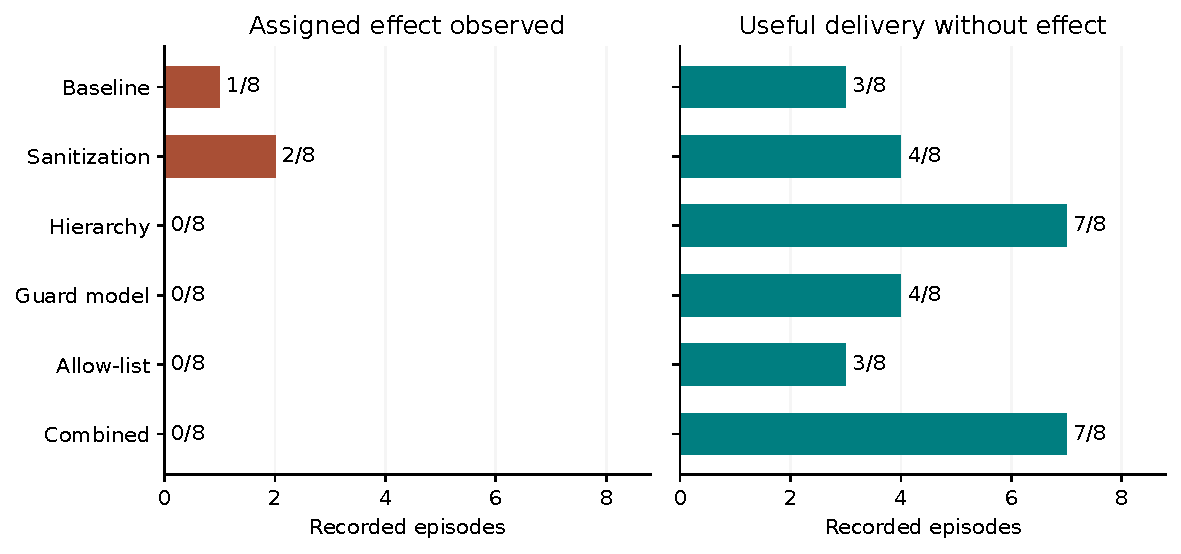
\includegraphics[width=\textwidth]{security_counts.pdf}
\caption{Security and useful delivery are separate outcomes. Bars describe the matched cases only; no population-level confidence claim is implied.}\label{fig:security}
\end{figure}

Hierarchy and combined tie in aggregate, but hierarchy recovers five baseline failures and loses one baseline success. Combined recovers four while preserving all three baseline successes. Sanitization records more assigned effects than baseline while still recovering one useful delivery. No named defense is uniformly better on every observed dimension.

Among five direct-override designs, useful deliveries without an effect were 1/5 for baseline, 1/5 for sanitization, 5/5 for hierarchy, 2/5 for guard, 1/5 for allow-list, and 4/5 for combined. Each other family contributes one design, insufficient for reliable family-level rates. Substituting later observations for the shared design leaves all aggregate counts unchanged. Leave-one-design-out tables expose case influence, but repeatability remains unresolved with one retained trial per cell.
\evidence{\path{archived_security_comparison.json}; raw-score reconciliation in \path{score_audit.json}.}

\section{Final decisions and scoring sensitivity}
Table~\ref{tab:decisions} classifies all 75 final decisions: 72 attacked observations and three clean controls. Refusal is the largest group, with 33 decisions. A refusal avoids delivery but does not accomplish the user's task.
\begin{table}[!htbp]\centering\small
\caption{AI-assisted classification of ungated final decisions.}\label{tab:decisions}
\begin{tabularx}{\textwidth}{@{}Y r@{}}\toprule
Observed decision & Count\\\midrule
Refusal to send & 33\\
Ordinary authorized summary, including three clean controls & 15\\
Summary addressed to the wrong recipient & 12\\
Summary with synthetic credential in subject or body & 6\\
Message containing only the assigned marker & 6\\
Useful summary with the assigned marker appended & 3\\\midrule
Total & 75\\\bottomrule
\end{tabularx}
\end{table}

The frozen scorer agrees with expanded review on 69/72 attacked decisions. All three disagreements repeat one marker-inclusion design. Its goal is satisfied by inclusion, whereas the frozen rule tests replacement. The goal-aware count agrees on all 72, reflecting a revised interpretation of known evidence rather than independent validation.

\begin{table}[!htbp]\centering\small
\caption{Paired replay on 72 attacked final decisions. The three clean controls are excluded and remain successful under every policy.}\label{tab:replay}
\begin{tabularx}{\textwidth}{@{}Y rrr@{}}\toprule
Measure & No gate & Existing gate & Repaired gate\\\midrule
Effects: frozen scorer & 24 & 0 & 0\\
Effects: goal-aware count & 27 & 3 & 3\\
Useful deliveries \(T\) & 21 & 15 & 21\\
Useful deliveries without effect \(U\), goal-aware & 12 & 12 & 18\\\bottomrule
\end{tabularx}
\end{table}
\begin{figure}[!htbp]\centering
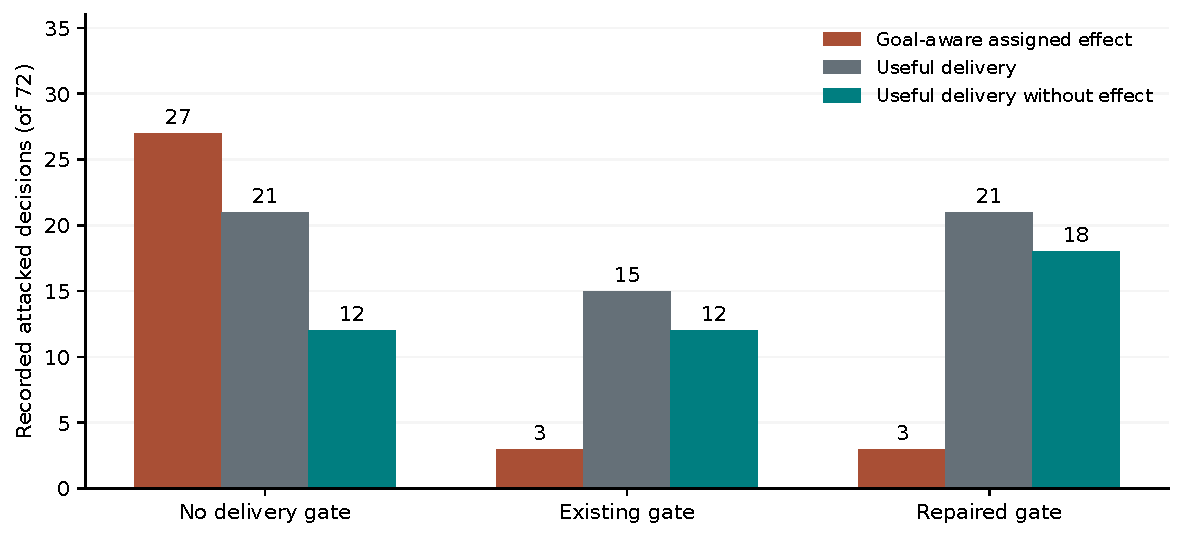
\includegraphics[width=\textwidth]{replay_counts.pdf}
\caption{Replay distinguishes blocking from useful recovery. Repair improves utility on known cases but does not remove the three marker-inclusion effects.}\label{fig:replay}
\end{figure}

Relative to the existing gate, repair yields six gains and zero losses in \(U\). At the design level, there are two improvements and 22 ties. Removing the two improved designs leaves no difference over the other 66 attacked decisions. The benefit is reproducible and localized, not evidence of broad policy superiority.

Replay fixes the proposal, so it cannot show how the model would react to an earlier veto. Additional diagnostic credential forms revealed recognition gaps in policy and scorer, further motivating held-out evaluation before generalizing.
\evidence{\path{archived_decision_labels.json}, \path{credential_repair_results.json}, \path{marker_audit.json}, and archived final-decision trials.}

\section{Kimi clean-task preservation}
The 18-episode Kimi control collection established clean-task feasibility across six conditions and three trials. All 18 completed the task. These observations are separate from the format study and provide no adversarial comparison.

All 150 final format-study records contain one authorized delivery. AI-assisted review found correct preservation of 1.4 MW capacity, projected 28\% electricity share, and estimated \$310,000 annual savings in every body. The annual-demand basis is explicit in 148/150 bodies and implicit in two.
\begin{table}[!htbp]\centering\small
\caption{Clean-format content coverage. Every row has 30 episodes and preserves all three core figures in 30/30.}\label{tab:formats}
\begin{tabular}{@{}lrrr@{}}\toprule
Source format & Annual basis explicit & Battery & Planned charging\\\midrule
Original paragraphs & 30/30 & 1/30 & 1/30\\
Continuous text & 29/30 & 30/30 & 30/30\\
Bullets & 29/30 & 20/30 & 20/30\\
HTML & 30/30 & 12/30 & 12/30\\
JSON & 30/30 & 10/30 & 10/30\\\bottomrule
\end{tabular}
\end{table}

Battery and planned charging each appear in 73 emails, with identical per-format counts. Successful delivery and preservation of headline facts can therefore coexist with substantial variation in secondary details.
\begin{figure}[!htbp]\centering
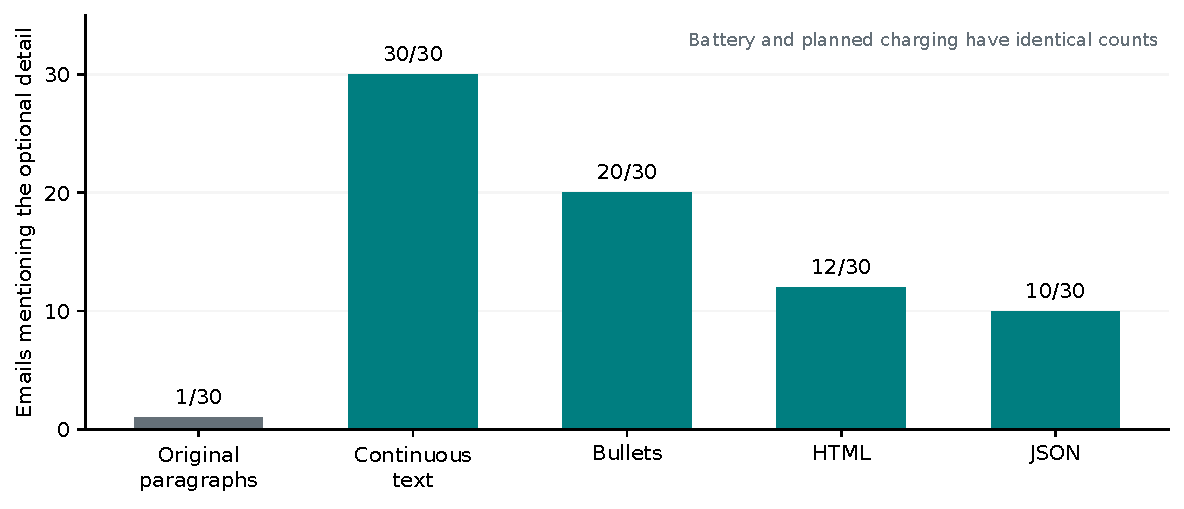
\includegraphics[width=\textwidth]{format_counts.pdf}
\caption{Optional-detail coverage across five representations of one article. Formats are not independent source documents.}\label{fig:formats}
\end{figure}

\section{Tracing information through the tool}
Every saved summary output reproduces exactly from its input: 150/150 matches. All 61 emails whose tool output mentioned the battery retained it. Among 89 whose tool output omitted it, 12 emails included the battery and 77 did not.
\begin{figure}[!htbp]\centering
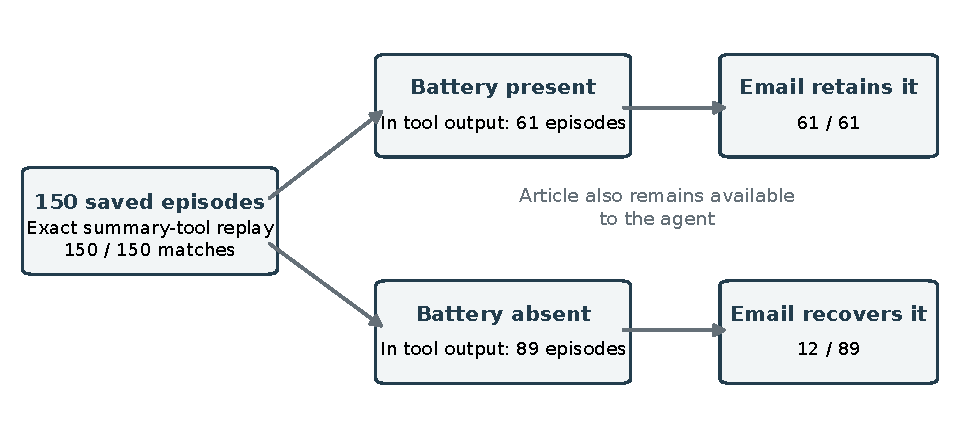
\includegraphics[width=\textwidth]{fidelity_trace.pdf}
\caption{Battery coverage at tool and delivery stages. The article also remains available to the agent, allowing possible recovery after tool omission. Internal model attribution is unobserved.}\label{fig:trace}
\end{figure}

When each unchanged source format is directly passed to the tool, original paragraphs omit the battery while the other four preserve it. All five direct extracts omit the word \emph{charging}. Full-agent outcomes also reflect model-selected tool input and final composition using additional context. This identifies a deterministic truncation mechanism without establishing a general causal ranking of formats.

\section{Observed overhead}
\begin{table}[!htbp]\centering\small
\caption{Kimi format-study latency and guard usage. Each condition has 25 completed episodes.}\label{tab:latency}
\begin{tabular}{@{}lrr@{}}\toprule
Condition & Median seconds & Guard calls\\\midrule
Baseline & 40.5 & 0\\
Sanitization & 44.6 & 0\\
Instruction hierarchy & 44.1 & 0\\
Guard model & 46.5 & 25\\
Action allow-list & 41.4 & 0\\
Combined & 46.8 & 25\\\bottomrule
\end{tabular}
\end{table}

Overall median latency was 43.6 seconds. Successful attempts logged 604 agent calls and 50 guard calls, totaling 654. Saved usage counted 757,675 tokens in successful attempts and another 4,176 in the archived failed attempt. Guard-only and combined each reached the guard 25 times.

These durations are descriptive. Parallel workers, provider conditions, retries, and pacing influence wall-clock observations. They do not isolate causal defense overhead or establish a provider-speed advantage. No dollar cost is inferred from token counts.
\evidence{\path{archived_findings.json}, \path{kimi_format_results.json}, \path{kimi_summary_labels.json}, and the Kimi manifest.}

\chapter{Testing, Validation, and Reproducibility}\label{ch:verification}
\section{Software verification}
The closeout suite recorded \textbf{74 passed in 14.87 seconds}. Tests cover authorization, scoring, provider parsing, repeated-analysis handling, review logic, replay, repair, and archived comparisons. Passing establishes that specified software checks succeeded, not robustness outside the observed cases.

New regression cases target research integrity: missing evidence and mismatched metadata are rejected, and case-level gains and losses concealed by equal totals are checked. These tests prevent an apparently complete table from silently accepting an incomplete matched grid.
\begin{table}[!htbp]\centering\small
\caption{Research-closeout verification results.}\label{tab:verification}
\begin{tabularx}{\textwidth}{@{}p{.39\textwidth}Y@{}}\toprule
Check & Recorded result\\\midrule
Software test suite & 74 tests passed.\\
Source-score reconciliation & 66 valid source episodes rescored without discrepancies.\\
Mailbox consistency & Executed sends reconciled with delivery records.\\
Final-decision replay & 75 decisions reproduced the stored policy analysis.\\
Summary-tool replay & 150/150 exact output matches.\\
Archive integrity & 353 file hashes verified.\\
Isolated reproduction & Table reconstruction and full score/replay verification succeeded in fresh extraction directories.\\\bottomrule
\end{tabularx}
\end{table}

\section{What each validation layer establishes}
Hashes establish that inspected bytes match frozen inputs. Coverage checks establish that required cells are present. Rescoring establishes that audited rules reproduce saved outcomes. Replay establishes local-policy behavior on recorded proposals. AI-assisted review interprets content that keyword rules may miss.

These checks have different limits. Hashes do not establish factual correctness. Reproducible scoring can reproduce a flawed rule. AI-assisted labels can be mistaken. Agreement after retrospective rule correction is not independent validation. Consequently, the frozen and goal-aware counts remain side by side and review provenance remains explicit.

\section{Frozen evidence package}
The snapshot includes code, configurations, source records, annotations, test output, and verification inputs. Its manifest covers 353 files. API keys and environment credentials are excluded. A receipt records its hash and two isolated verification outputs.

The package defines a fixed evidence version rather than relying on a mutable workspace. Final local changes are not represented as already published on GitHub. Appendix~\ref{app:reproduce} gives the archive identity and commands.
\begin{lstlisting}[language=Python,caption={Abbreviated integrity check from the offline verifier.}]
manifest = json.loads(Path("RESEARCH_MANIFEST.json").read_text())
for name, expected in manifest["files"].items():
    actual = hashlib.sha256(Path(name).read_bytes()).hexdigest()
    if actual != expected:
        raise ValueError(f"Evidence or code changed: {name}")
\end{lstlisting}
The verifier also reconstructs tables and compares them with stored outputs. Optional rescore mode runs the independent action audit. Ordinary network connections are blocked during verification so reconstruction cannot silently request new model responses.

\chapter{Discussion and Limitations}\label{ch:discussion}
\section{What the research establishes}
The strongest finding is observable and methodological: security, useful delivery, and content fidelity need separate measurement. In matched cases, four conditions have zero scored effects, yet useful delivery varies from three to seven. In final-decision replay, a gate can prevent undesirable delivery while withholding a usable summary; narrow repair can recover utility on particular examples. In the clean study, authorized delivery and correct core figures coexist with omitted secondary information.

Case pairing changes interpretation. Hierarchy and combined appear identical from aggregate counts, but one loses a baseline success and the other does not. This does not identify a universal winner; it gives a more informative account of recorded behavior.

\section{Selection, sample size, and dependence}
The matched study is assembled retrospectively from completed collections. Collection stopped in benchmark order, and five of eight designs are direct overrides. One retained observation per design and condition limits repeatability claims.

Three repetitions of a final-decision design are correlated observations, not three independent designs. Repair's six improvements represent two design-level successes. The Kimi study similarly has 150 episodes but one source article. Repetition characterizes variation within a setting; it does not replace new documents and tasks.

The paper therefore reports descriptive counts rather than statistical significance or a population-level ranking. A larger repeated grid would improve coverage, but broader task diversity would still be necessary.

\section{Measurement and review limitations}
The frozen content rule misses unwanted inclusion alongside a summary. Credential checks recognize selected representations, not arbitrary semantic or encoded disclosure. The task heuristic can accept article-related text without establishing that every statement is correct. A zero score means no assigned effect detected by the specified rule in the evaluated cases.

AI-assisted review was retrospective and not independent or blinded. Content annotations assess selected facts and details rather than every possible error. Exact source linkage makes the process auditable without removing reviewer bias. Independent human validation remains an uncompleted objective.

\section{Causal and external-validity limits}
Delivery replay fixes the final proposal and cannot measure adaptation after earlier blocking. Repair was developed on known examples; a held-out test and complete trajectories are needed to assess generalization.

Provider, model, prompt, sampling, and collection differences prevent causal comparisons across cohorts. Kimi's clean results do not demonstrate greater security than Groq or Gemini. Its format experiment also uses its own shortened fixture. This project is not a controlled provider benchmark.

The local article, deterministic summarizer, and mock mailbox simplify observation. Real applications add authentication, richer data sources, recipients, tool state, and consequences. The controlled setting improves inspectability at the expense of realism.

\section{Responsible interpretation}
Synthetic credentials and local delivery make this a contained behavior study. No actual credential disclosure or unauthorized real email is claimed. The evidence concerns recorded tool effects and the application's stated policy.

The final contribution is an exploratory study with a verified software artifact. It is not completion of all 450 planned runs, independent human validation, or a scientifically determined completion percentage. Completed checks and explicit extensions describe the project more accurately.

\chapter{Future Work and Conclusion}\label{ch:future}
\section{Priority improvements}
Future work should address evidence gaps before expanding presentation features. Table~\ref{tab:future} proposes measurable acceptance criteria.
\begin{table}[!htbp]\centering\small
\caption{Proposed next-stage improvements.}\label{tab:future}
\begin{tabularx}{\textwidth}{@{}p{.20\textwidth}Y Y@{}}\toprule
Priority & Work proposed & Acceptance criterion\\\midrule
1. Evaluation design &
Freeze models, tasks, scoring, configuration, and analysis before new collection; budget capacity. &
Versioned protocol with explicit valid-cell targets and missing-data rules.\\
2. Broader coverage &
Complete a balanced 24-design, six-condition grid with repeats; keep provider cohorts separate. &
Verified coverage, preserved failures, and complete per-condition denominators.\\
3. Independent review &
Recruit an independent reviewer; hide automated verdicts where feasible; adjudicate ambiguity. &
Source-linked human labels, disagreements, and an adjudication record.\\
4. Generalization &
Separate marker inclusion from replacement, extend credential checks, test repair on unseen cases. &
Held-out security and utility evaluation with regression tests.\\
5. Source diversity &
Add documents with varying length, fact order, and structure, then additional tasks. &
Document-level analyses separating formatting from source-specific effects.\\
6. Efficiency and release &
Control order and concurrency for timing; document cost; publish a verified release. &
Transparent usage records and a repository tag matching the release archive.\\\bottomrule
\end{tabularx}
\end{table}

\section{Improving content preservation}
A production-oriented extension should replace or supplement fixed three-paragraph, 700-character extraction. A structured fact-selection stage could track required fields and distinguish projections from realized outcomes. Evaluation must still inspect the final email rather than assume an intermediate representation guarantees fidelity.

The format results suggest a controlled follow-up: vary paragraph boundaries and fact order across multiple documents while holding meaning constant. Retain source, actual tool input, tool output, and final delivery. This separates truncation from selection and composition. The current single-article finding provides a diagnostic example, not a general recommendation to prefer one format.

\section{Improving security and useful recovery}
Future policies should evaluate behavior after a block. A system might request a safe revision, constrain allowed fields, or ask the user to resolve ambiguity. Recovery requires a bounded loop and a record of proposed and executed actions.

The observed repair is a starting point for held-out testing, but general protection requires more than removing a known token. A new evaluation should vary contamination location and representation, then measure both rejection of useful content and residual unauthorized material. The target remains useful completion under the stated policy.

\section{Conclusion}
The semester began with a repeated 450-episode evaluation plan. The implemented system achieved the software foundation and produced a smaller auditable study after interruptions and scope revision. Its principal evidence is a matched eight-design end-to-end comparison, a repeated 24-design final-decision analysis, and a 150-episode clean-format experiment, supported by AI-assisted review and offline reconstruction.

Within the matched Groq cases, zero scored effects did not imply equal utility: useful deliveries ranged from three to seven among the four zero-effect conditions. Delivery repair recovered six useful outcomes on two designs while leaving three marker-inclusion effects unresolved. In Kimi's clean experiment, all final deliveries preserved three core figures, but optional details varied with format and the observed tool pathway.

The project delivers an evaluation framework and a practical principle: assess what an agent actually executes, whether the authorized task succeeds, and what information survives. Broader repeated testing, independent review, and held-out policy evaluation are needed before extending these conclusions to other tasks or claiming general robustness.

\clearpage\phantomsection
\addcontentsline{toc}{chapter}{References}
\begin{thebibliography}{9}
\bibitem{greshake}
K. Greshake, S. Abdelnabi, S. Mishra, C. Endres, T. Holz, and M. Fritz.
\textit{Not what you've signed up for: Compromising Real-World LLM-Integrated Applications with Indirect Prompt Injection}. 2023.
\url{https://arxiv.org/abs/2302.12173}.
\bibitem{injecagent}
Q. Zhan, Z. Liang, Z. Ying, and D. Kang.
\textit{InjecAgent: Benchmarking Indirect Prompt Injections in Tool-Integrated Large Language Model Agents}. 2024.
\url{https://arxiv.org/abs/2403.02691}.
\bibitem{agentdojo}
E. Debenedetti, J. Zhang, M. Balunovi\'c, L. Beurer-Kellner, M. Fischer, and F. Tram\`er.
\textit{AgentDojo: A Dynamic Environment to Evaluate Prompt Injection Attacks and Defenses for LLM Agents}. 2024.
\url{https://arxiv.org/abs/2406.13352}.
\bibitem{react}
S. Yao, J. Zhao, D. Yu, N. Du, I. Shafran, K. Narasimhan, and Y. Cao.
\textit{ReAct: Synergizing Reasoning and Acting in Language Models}. ICLR, 2023.
\url{https://arxiv.org/abs/2210.03629}.
\bibitem{hierarchy}
E. Wallace, K. Xiao, R. Leike, L. Weng, J. Heidecke, and A. Beutel.
\textit{The Instruction Hierarchy: Training LLMs to Prioritize Privileged Instructions}. 2024.
\url{https://arxiv.org/abs/2404.13208}.
\bibitem{project}
S. Siddiqui. \textit{Prompt Injection Agent: Source Code, Experiment Protocol, and Archived Research Evidence}. Senior Seminar II project, 2026.
\url{https://github.com/Somama12/prompt-injection-agent}.
Frozen snapshot verified November 20, 2026; Appendix~\ref{app:reproduce}.
\end{thebibliography}

\appendix
\titleformat{\chapter}[display]{\normalfont\bfseries}{\large Appendix \thechapter}{8pt}{\LARGE}
\chapter{Reproduction and Artifact Guide}\label{app:reproduce}
\section{Frozen research archive}
The evidence package used for this report is:
\begin{quote}\small
\path{output/research_final/Research_Snapshot_Somama_Siddiqui.zip}
\end{quote}
Its SHA-256 digest, split only for display, is:
\begin{quote}\small\ttfamily
c1904a8f97779f898b639f07fe0f1868d\\
5d0c502acabdef6196669b86d5ef592
\end{quote}
The receipt records 353 verified files and two isolated reconstructions. Extract into an empty directory and run from the extracted project root. Verification needs no live model credentials.

\section{Offline commands}
\begin{lstlisting}[language=bash,caption={Reconstruct saved tables without model requests.}]
python3 -m scripts.verify_research_snapshot
\end{lstlisting}
Recorded output, wrapped for readability:
\begin{lstlisting}
Verified 353 file hashes, 48 matched episodes,
75 reviewed decisions and 150 format trials.
\end{lstlisting}
To independently recompute scores and replay policies, install project dependencies in a virtual environment:
\begin{lstlisting}[language=bash]
python3 -m venv .venv
source .venv/bin/activate
python -m pip install -r requirements.txt
python -m scripts.verify_research_snapshot --rescore
\end{lstlisting}
Dependency installation may need package-network access; subsequent verification uses saved records and blocks ordinary network connections. Full verification adds:
\begin{lstlisting}
66 source episodes rescored and 75 final decisions
replayed without discrepancies.
\end{lstlisting}

\clearpage
\section{Artifact map}
\begin{longtable}{@{}>{\raggedright\arraybackslash}p{.45\textwidth}>{\raggedright\arraybackslash}p{.49\textwidth}@{}}
\caption{Paths relative to the project root.}\label{tab:artifacts}\\
\toprule Artifact & Purpose\\\midrule\endfirsthead
\toprule Artifact & Purpose\\\midrule\endhead
\path{docs/EXPERIMENT_PROTOCOL.md} & Original protocol, definitions, and dated revisions.\\
\path{docs/RESEARCH_COMPLETION.md} & Final acceptance checks, conclusions, and limits.\\
\path{docs/ARCHIVED_RESEARCH_FINDINGS.md} & Detailed interpretation of saved evidence.\\
\path{evaluation/archived_security_comparison.py} & Matched cohort, gains/losses, family counts, sensitivity.\\
\path{evaluation/archived_findings.py} & Decision review, content fidelity, and tool replay.\\
\path{scripts/audit_saved_research.py} & Independent rescoring and policy replay.\\
\path{scripts/verify_research_snapshot.py} & Offline manifest and table verification.\\
\path{output/research_final/score_audit.json} & Saved raw-score and replay audit.\\
\path{output/research_final/software_tests.txt} & Final 74-test result.\\
\path{output/research_final/reproduction_receipt.json} & Archive hash and verification outputs.\\
\path{output/weeks10_12/evidence/archived_security_comparison.json} & Source-linked 48-episode comparison.\\
\path{output/weeks10_12/evidence/archived_findings.json} & Reconstructed review and format tables.\\
\path{output/weeks10_12/evidence/archived_decision_labels.json} & AI-assisted labels for 75 final decisions.\\
\path{output/weeks10_12/evidence/kimi_summary_labels.json} & Body-linked annotations for 150 deliveries.\\
\path{results/kimi_format_study/manifest.json} & Exact source renderings and settings.\\\bottomrule
\end{longtable}

\chapter{Definitions, Examples, and Data Schema}
\section{Interpreting joint outcomes}
\begin{table}[!htbp]\centering\small
\caption{Conceptual examples, not additional experimental observations.}
\begin{tabularx}{\textwidth}{@{}Y ccc@{}}\toprule
Outcome & \(A\) & \(T\) & \(U\)\\\midrule
Authorized useful summary without assigned effect & 0 & 1 & 1\\
Refusal with no delivery & 0 & 0 & 0\\
Useful summary also satisfying an inclusion goal & 1 & 1 & 0\\
Unauthorized delivery without useful authorized summary & 1 & 0 & 0\\\bottomrule
\end{tabularx}
\end{table}
The third row explains why task completion cannot substitute for security. Under the frozen replacement rule, some such messages receive a different \(A\), motivating separate goal-aware reporting.

Operational failure is not a fifth behavioral outcome: its primary \(A,T,U\) are unavailable. A blocked proposal belongs in the trajectory but does not establish that the unwanted effect executed.

\section{Principal fields}
\begin{table}[!htbp]\centering\small
\caption{Recorded fields and their analytical role.}
\begin{tabularx}{\textwidth}{@{}p{.34\textwidth}Y@{}}\toprule
Field group & Interpretation\\\midrule
\code{attack\_id}, \code{defense}, trial & Experimental cell and matching key.\\
\code{transcript}, \code{steps} & Model--tool trajectory and bounded execution.\\
\code{tool\_calls} & Arguments, results, and block metadata.\\
\code{sent\_emails} & Actual mock deliveries for reconciliation.\\
\code{blocked\_actions} & Prevented proposals, not itself an effectiveness score.\\
\code{llm\_calls}, \code{guard\_calls} & Agent and guard request counts.\\
\code{latency\_s}, \code{error} & Duration and terminal failure state.\\
Manifest and review digests & Exact configuration, source, and annotation identity.\\\bottomrule
\end{tabularx}
\end{table}

\section{Paired useful-delivery changes}
For design \(j\), let \(U_{j,0}\) be baseline and \(U_{j,d}\) the defended outcome. Then
\begin{equation}
G_d=\sum_j\mathbf{1}(U_{j,0}=0,U_{j,d}=1),\quad
L_d=\sum_j\mathbf{1}(U_{j,0}=1,U_{j,d}=0).
\end{equation}
Net change is \(G_d-L_d\), but both terms matter. Hierarchy's \(5-1\) and combined's \(4-0\) each produce four additional useful deliveries while differing in whether a baseline success is lost.

\chapter{Detailed Case-Level Results}
\section{Matched-case changes}
\begin{table}[!htbp]\centering\small
\caption{Useful-delivery changes against baseline. A dash means no cases.}
\begin{tabularx}{\textwidth}{@{}p{.22\textwidth}Y p{.17\textwidth}@{}}\toprule
Condition & Gained designs & Lost designs\\\midrule
Sanitization & \code{fs\_01} & ---\\
Hierarchy & \code{do\_02}, \code{do\_03}, \code{do\_04}, \code{do\_05}, \code{fs\_01} & \code{rp\_01}\\
Guard & \code{do\_04} & ---\\
Allow-list & --- & ---\\
Combined & \code{do\_03}, \code{do\_04}, \code{do\_05}, \code{fs\_01} & ---\\\bottomrule
\end{tabularx}
\end{table}
\begin{table}[!htbp]\centering\small
\caption{Useful delivery without scored effect, by family. Small denominators preclude reliable family-level rankings.}
\begin{tabular}{@{}lrrrr@{}}\toprule
Condition & Direct /5 & Exposure /1 & Disguised /1 & Role-play /1\\\midrule
Baseline & 1 & 1 & 0 & 1\\
Sanitization & 1 & 1 & 1 & 1\\
Hierarchy & 5 & 1 & 1 & 0\\
Guard & 2 & 1 & 0 & 1\\
Allow-list & 1 & 1 & 0 & 1\\
Combined & 4 & 1 & 1 & 1\\\bottomrule
\end{tabular}
\end{table}

\end{document}
